\chapter{Architectural Design}

\section{Overview}
The CKB platform system is composed by a 3-tier architecture.\\
Its software application architecture is organized into three logical tiers: the presentation tier, or user interface; the application tier, where data is processed; and the data tier, where the data associated with the application is stored and managed.

\begin{figure}[H]
    \centering
    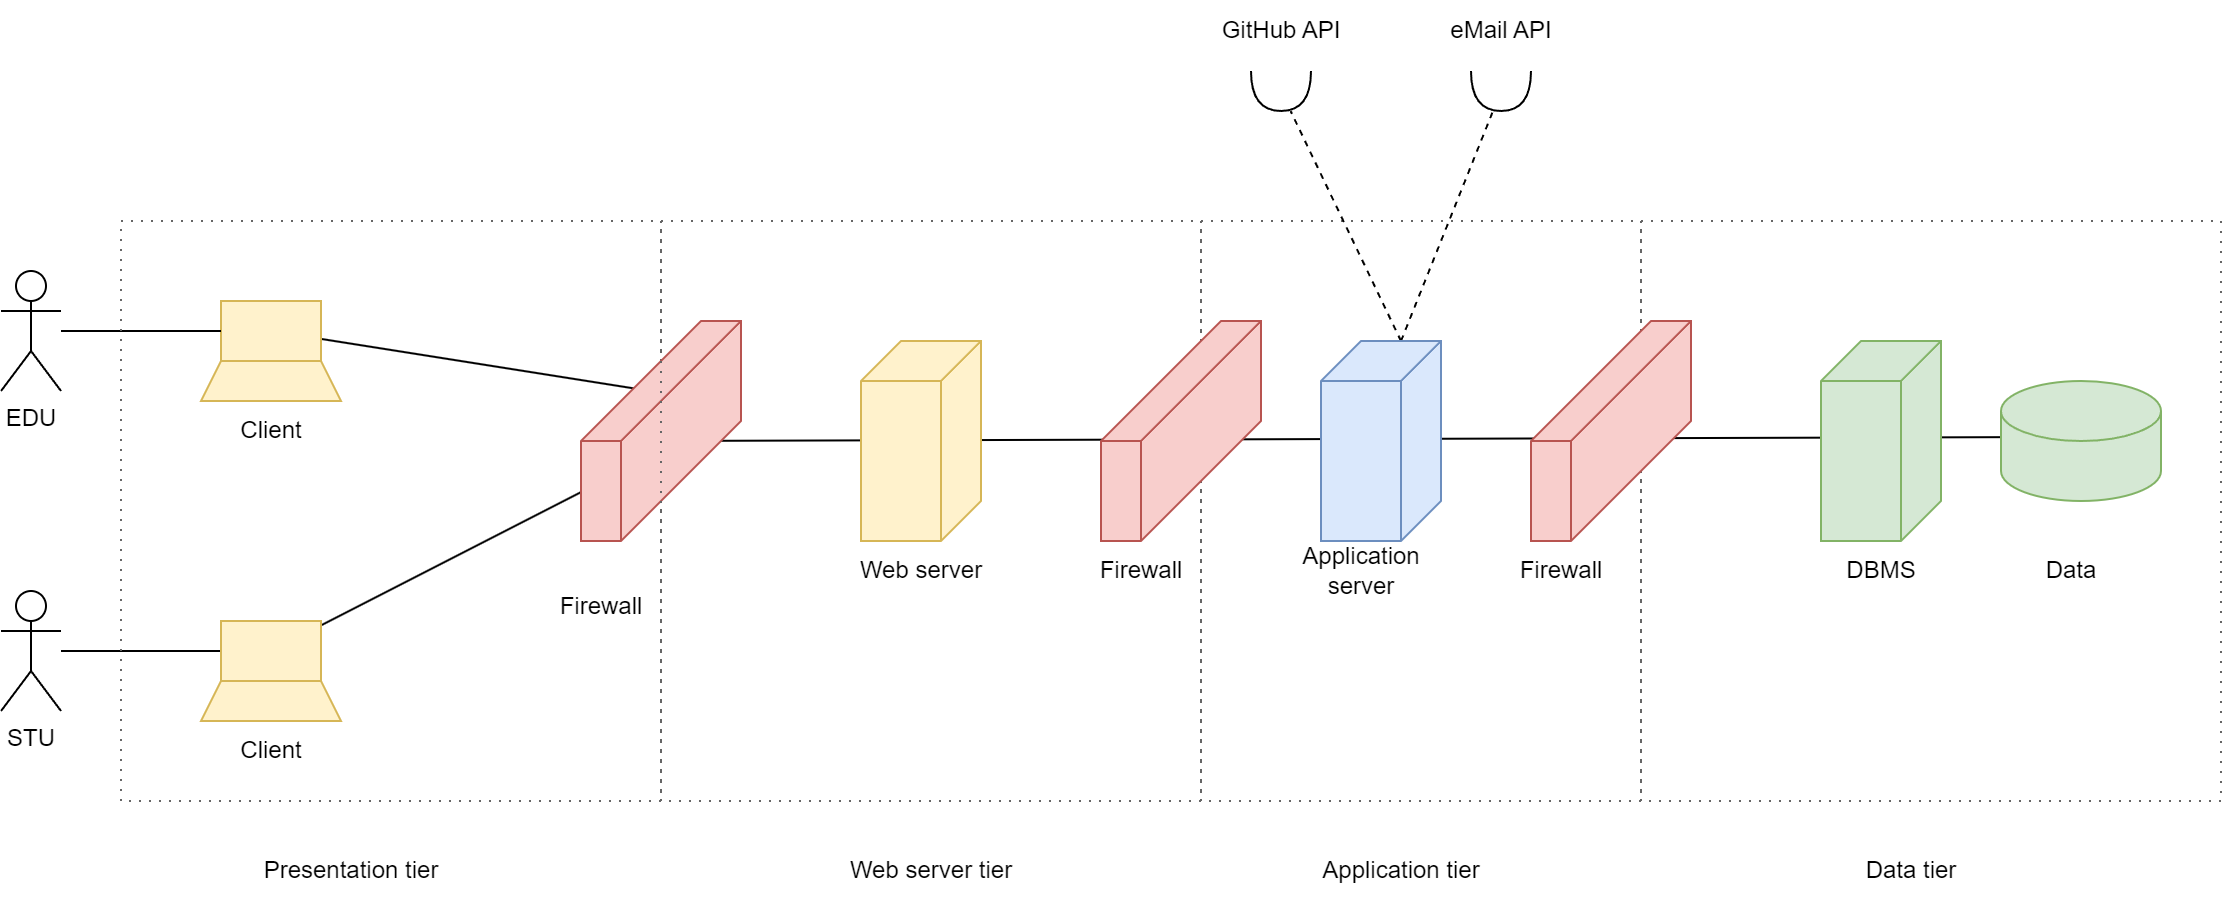
\includegraphics[width=\textwidth]{images/diagrams/high_level_diagram.png}
    \caption{High level components diagram}
\end{figure}

The service will be accessed through a web interface, employing a Single Page Application (SPA). Utilizing an SPA is ideal for this application, as it facilitates extensive interaction without necessitating frequent page reloads.\\
The system's architecture is structured into distinct layers, with application servers interacting with a database management system and utilizing APIs for data retrieval and storage. {\color{red}Adhering to REST standards, the application servers are intentionally designed to be stateless, -e le sessioni di log in come ce le gestiamo?-} while the system will include more than one firewall to ensure security.\\

\section{Component view}
The system is composed by the following components:

\begin{figure}[H]
    \centering
    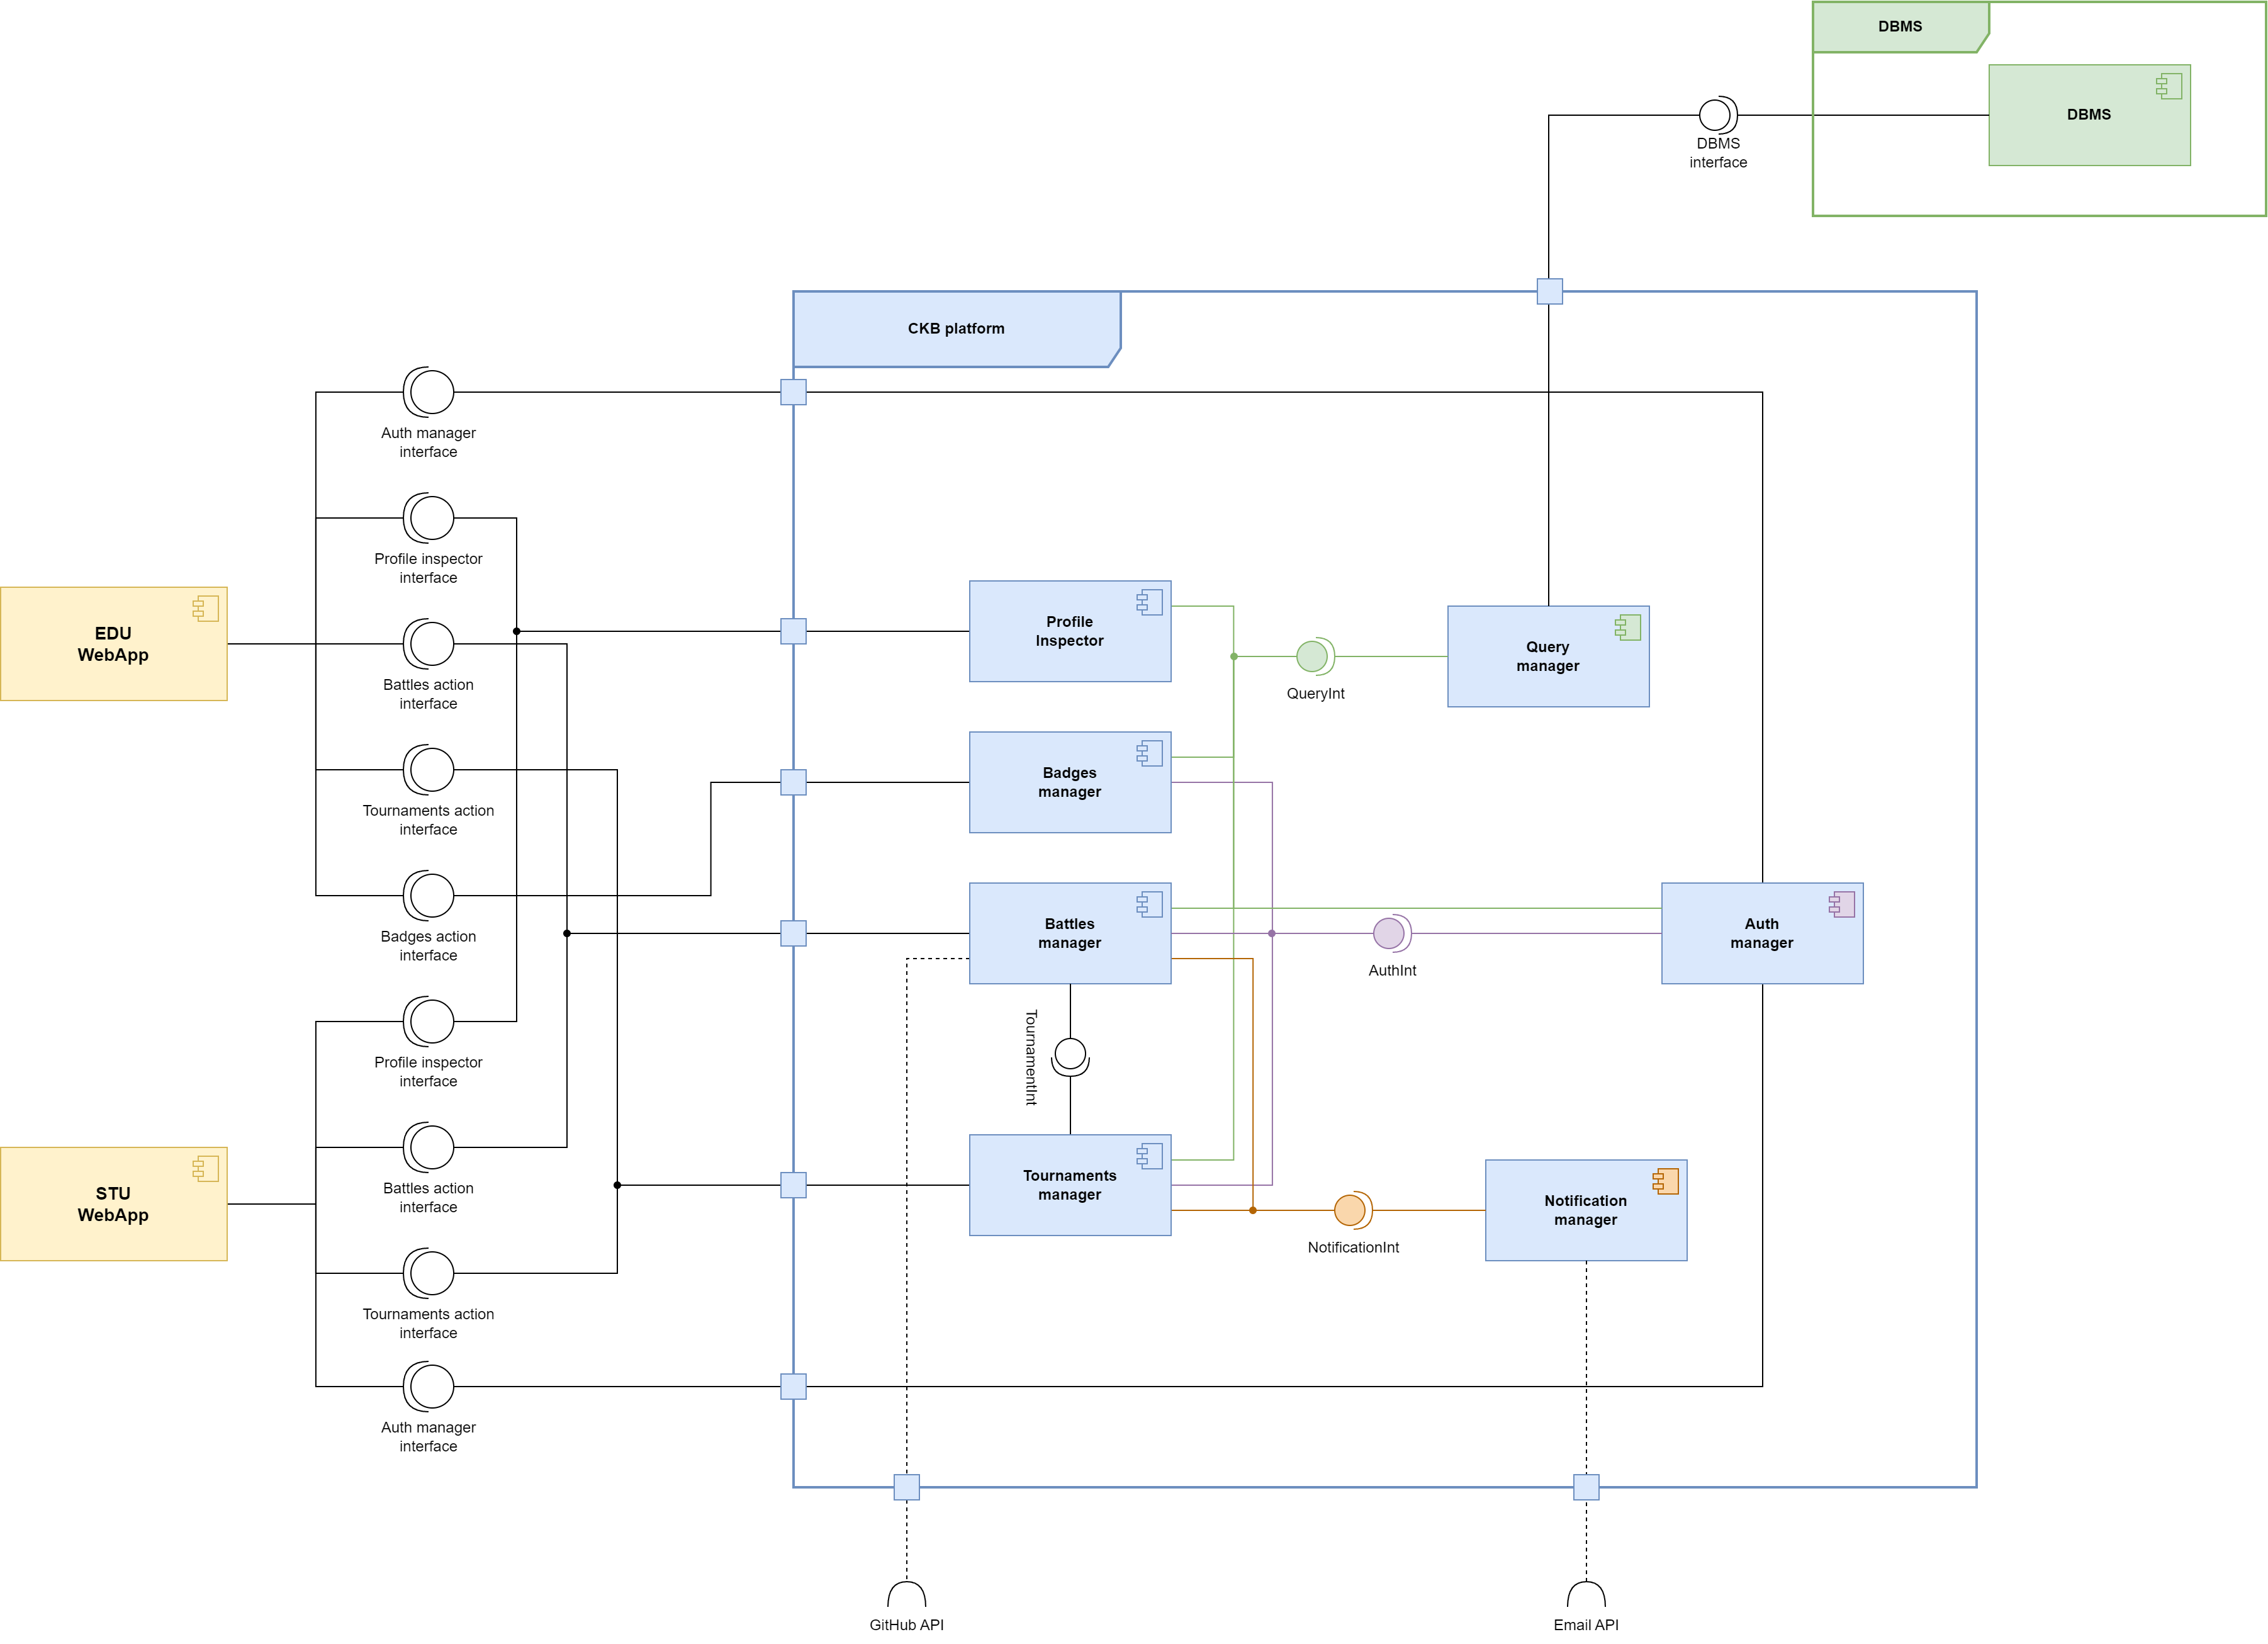
\includegraphics[width=\textwidth]{images/diagrams/component_diagram.png}
    \caption{Component diagram}
\end{figure}

{\color{red}Qui va bene aver raggruppato le interfacce oppure vanno messe singolarmente, una per ogni endpoint?}

\subsection*{Query manager}
The query manager is the component that handles the queries made by the other components that need to access the database. It is responsible for the execution of the queries and for the communication with the database.\\
It is interfaced with all the internal models of the system that need to access the database, i.e. all the other components of the system exept for the notification manager.\\
It is interfaced with the database through the DBMS API, external to the system.\\

\subsection*{Auth manager}
The auth manager is the component that handles the authentication of the users and the authorization of the requests made by the other components that need to access the database with respect to the user that made the request.\\
It is interfaced with all the internal models of the system that behave differently depending on the level of the user that made the request, i.e. the badges manager, the tournament manager and the battle manager.\\
It isn't interfaced with any external component.\\

\subsection*{Notification manager}
The notification manager is the component that handles the need of the system to notify the users of some events, such as the start of a tournament or the end of a battle.\\
It is interfaced with all the internal models of the system that need to notify the users, i.e. the tournament manager and the battle manager.\\
It is interfaced with the Email API, external to the system.\\

\subsection*{Badges manager}
The badges manager is the component that handles the gamification badges.\\
It allows:
\begin{itemize}
    \item the creation of new badges;
    \item the assignment of badges to the STUs;
    \item the visualization of the badges assigned to a user.
\end{itemize}
{\color{red}Qui devo interfacciare anche con battle e user?}
It is interfaced with the auth manager (since the creation of a badge is admissible only for the EDUs) and with the query manager (since it needs to access the database to store the badges).\\

\subsection*{Tournament manager}
The tournament manager is the component that handles the creation and the management of the tournaments.\\
It allows: